\chapter{Results and Analysis}
\label{ch:results}

This chapter reports what the experiments found. Each section takes one
question, states the comparison that answers it, and gives the result with a
95\% confidence interval resampled by conversation. The chapter moves from the
accounting question (what should be budgeted), through the core decision
(select or compress), the choice of scorer and its transfer, to end-task
accuracy, comparison with existing memory designs, scale, and finally the
behaviour of the complete application. It closes with the standards that were
followed to make the results valid and reproducible. Unless stated otherwise,
the context budget is $B=2048$ tokens and answer recall is the primary metric
(Section~\ref{sec:metrics}).

\section{Storage was never budgeted}
\label{sec:accounting}

Work in this area caps the context assembled for each query and leaves the
store unbounded, and at first so did this project. Under that accounting a
store-everything baseline pays nothing to hold all 419 turns of a
conversation, so forgetting can only ever lose information. When our own
ablation was run that way, it reported the tiering and compression machinery
as a net loss against keeping everything and retrieving. Given how cost was
being counted, that verdict was correct.

A storage budget $S$ changes the question from what fits in the context to
what is worth keeping at all. Table~\ref{tab:storage} sweeps $S$ with the
context budget fixed at 2048 tokens, and the ranking under this accounting is
not the ranking under the old one. This is the most consequential observation
of the project: a protocol that leaves out a cost ends up answering a
different question from the one it seems to ask.

\section{Selection pays; compression does not}
\label{sec:selection}

Table~\ref{tab:storage} reports both metrics across the sweep, and
Fig.~\ref{fig:frontier} plots them. P1-S, which drops the lowest-utility item
when the cap binds, leads on answer recall at every budget. P1-A, which
compresses that item instead, leads on evidence recall at every budget, and
yet at $S=8192$ it falls behind even RAG on answer recall, by 3.4 points.

Here the identifier problem of Section~\ref{sec:metrics} shows up in real
numbers. A demoted gist keeps the evidence identifiers of a turn whose text is
gone. Judged on evidence recall alone, compression looks like the better use
of a bounded store; checked for whether the answer text survived, it looks
like the worse one.

\begin{table}[htbp]
\caption[Recall against the storage budget $S$ in tokens, context budget 2048.]{Recall against the storage budget $S$ in tokens, context budget 2048.
$\Delta$ is P1-S minus RAG on answer recall: identical storage, fidelity and
retrieval, differing only in which turns are forgotten.}
\label{tab:storage}
\centering
\fontsize{10}{12}\selectfont
% GENERATED by paper/make_tables.py -- do not edit by hand.
\begin{tabular}{@{}rrrrrrrr@{}}
\toprule
& \multicolumn{3}{c}{Evidence recall (\%)} & \multicolumn{3}{c}{Answer recall (\%)} & \\
\cmidrule(lr){2-4}\cmidrule(lr){5-7}
$S$ & RAG & P1-A & P1-S & RAG & P1-A & P1-S & $\Delta$ \\
\midrule
1024 & 4.3 & 9.3 & 5.3 & 9.1 & 11.9 & \textbf{15.8} & \textbf{$+6.7$} \\
2048 & 10.1 & 19.4 & 11.8 & 18.3 & 22.7 & \textbf{27.8} & \textbf{$+9.5$} \\
4096 & 17.8 & 31.8 & 20.2 & 28.1 & 30.3 & \textbf{37.5} & \textbf{$+9.4$} \\
8192 & 30.6 & 45.6 & 38.6 & 44.3 & 41.0 & \textbf{57.8} & \textbf{$+13.4$} \\
16384 & 53.3 & 58.2 & 57.9 & 66.4 & 63.1 & \textbf{71.3} & \textbf{$+4.9$} \\
\bottomrule
\end{tabular}

\end{table}

\begin{figure}[htbp]
\centering
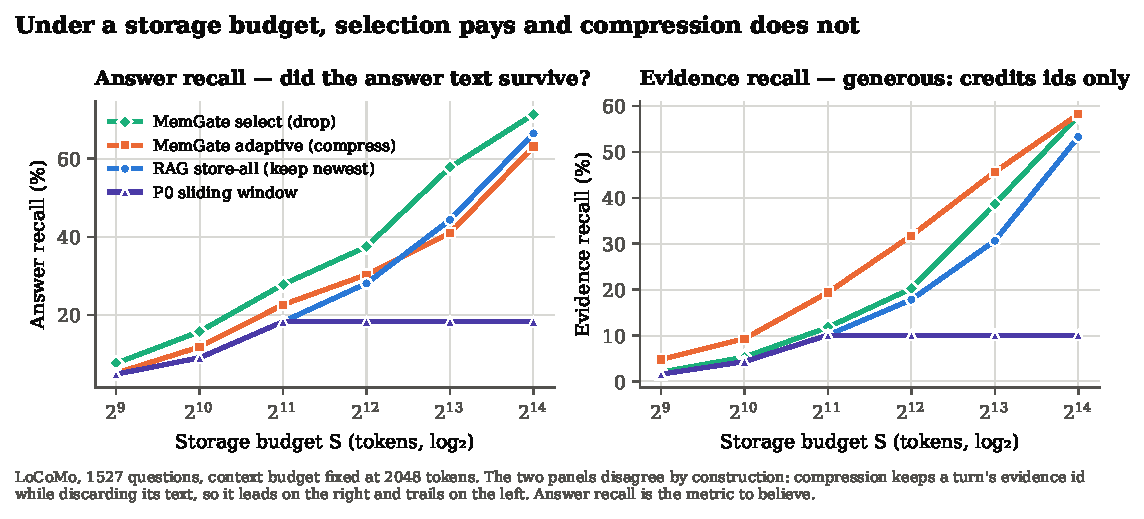
\includegraphics[width=0.85\textwidth]{../paper/figures/fig1_storage_frontier.pdf}
\caption{Recall against the storage budget for RAG, P1-A (compress) and P1-S
(drop).}
\label{fig:frontier}
\end{figure}

\section{Statistical significance}
\label{sec:significance}

Table~\ref{tab:significance} gives each contrast with intervals resampled by
conversation. Scored eviction beats FIFO on answer recall by $+9.37$ points,
and the interval excludes zero. The matching evidence-recall gain of $+2.42$
points does not survive clustering ($p=0.08$), so it is not claimed. It is
still reported, because a claim that fails a correctness check says something
useful about the check. The P1-S versus P1-A rows put signs on the divergence:
$+7.13$ on answer recall and $-11.53$ on evidence recall, both significant. The
two metrics disagree about direction, not just size.

\begin{table}[htbp]
\caption[Paired bootstrap (10{,}000 resamples) by conversation, with exact McNemar, at $S=4096$.]{Paired bootstrap (10{,}000 resamples) by conversation, with exact
McNemar, at $S=4096$. The second row is the claim we decline to make.}
\label{tab:significance}
\centering
\fontsize{10}{12}\selectfont
\begin{adjustbox}{max width=\textwidth}% GENERATED by paper/make_tables.py -- do not edit by hand.
\begin{tabular}{@{}llrcrc@{}}
\toprule
Comparison & Metric & $\Delta$ (pts) & 95\% CI (clustered) & McNemar $p$ & \\
\midrule
P1-S vs.\ RAG (FIFO) & answer & {\boldmath$+9.37$} & $[+5.45,\, +14.90]$ & $2.8\!\times\!10^{-5}$ & $\checkmark$ \\
P1-S vs.\ RAG (FIFO) & evidence & $+2.42$ & $[-1.48,\, +6.43]$ & 0.08 & \textsc{n.s.} \\
P1-S vs.\ P1-A (compress) & answer & {\boldmath$+7.13$} & $[+4.32,\, +10.28]$ & $2.1\!\times\!10^{-5}$ & $\checkmark$ \\
P1-S vs.\ P1-A (compress) & evidence & {\boldmath$-11.53$} & $[-14.73,\, -8.47]$ & $1.8\!\times\!10^{-23}$ & $\checkmark$ \\
P1-S vs.\ P0 (recency) & answer & {\boldmath$+19.16$} & $[+15.42,\, +24.13]$ & $8.2\!\times\!10^{-19}$ & $\checkmark$ \\
P1-S vs.\ P0 (recency) & evidence & {\boldmath$+10.15$} & $[+6.58,\, +13.84]$ & $1.2\!\times\!10^{-15}$ & $\checkmark$ \\
\bottomrule
\end{tabular}
\end{adjustbox}
\end{table}

\section{The rate--distortion crossover is not reached}
\label{sec:scaling}

Rate--distortion reasoning says compression must win eventually: compress a
record of everything far enough and it should beat a faithful record of only
part of it \cite{colaco2026rd}. Shrinking $S$ cannot test this, because every
policy hits the floor first, near 0.2\% evidence recall at $S=256$. The
missing axis is length, so up to ten LoCoMo conversations (186K tokens) were
concatenated with $S$ fixed, raising the compression ratio to $182\times$.
Table~\ref{tab:scaling} and Fig.~\ref{fig:scalingfig} show no crossover: the
margin of selection over compression narrows but stays positive, and the best
operating point stays at the vertex, a subset kept at full fidelity.

A concatenated stream is not a natural long conversation: each question is
about one piece and the rest act as distractors. This is therefore a stress
test of retention rather than a long-dialogue benchmark, and the crossover is
ruled out only along this axis and up to this ratio.

\begin{table}[htbp]
\caption[Answer recall (\%) against compression ratio at $S=2048$.]{Answer recall (\%) against compression ratio at $S=2048$. The last
column is the margin of dropping over compressing.}
\label{tab:scaling}
\centering
\fontsize{10}{12}\selectfont
% GENERATED by paper/make_tables.py -- do not edit by hand.
\begin{tabular}{@{}rrrrr@{}}
\toprule
Ratio & RAG & P1-A & P1-S & P1-S $-$ P1-A \\
\midrule
9$\times$ & 18.3 & 22.7 & \textbf{27.8} & $+5.2$ \\
18$\times$ & 10.8 & 13.0 & \textbf{18.9} & $+5.9$ \\
45$\times$ & 7.8 & 10.3 & \textbf{11.6} & $+1.3$ \\
91$\times$ & 4.6 & 7.4 & \textbf{8.7} & $+1.3$ \\
\bottomrule
\end{tabular}

\end{table}

\begin{figure}[htbp]
\centering
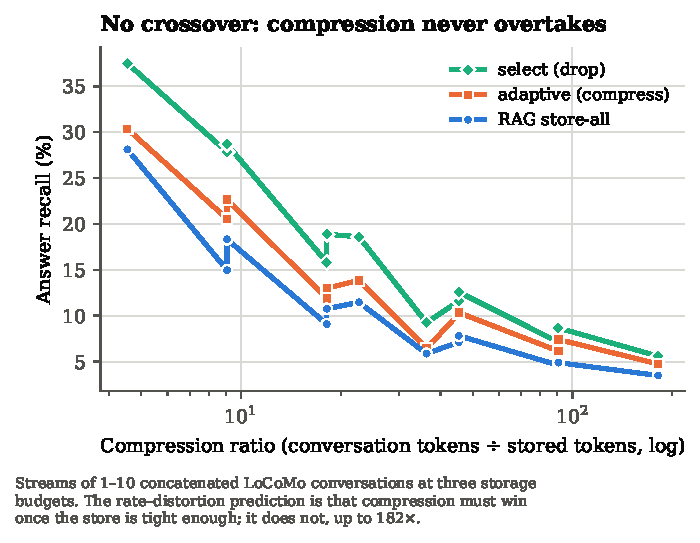
\includegraphics[width=0.85\textwidth]{../paper/figures/fig2_scaling.pdf}
\caption{Answer recall as the compression ratio grows to $182\times$.}
\label{fig:scalingfig}
\end{figure}

\section{The embedding index is not free}
\label{sec:bytes}

Counting storage in text tokens ignores the index that makes retrieval
possible. A 384-dimensional \texttt{float32} vector occupies 1{,}536\,B, while
a LoCoMo turn averages about 130\,B of text, so the index outweighs the content
it indexes by roughly a factor of 12, and the limiting resource becomes the
number of stored items rather than their length. Table~\ref{tab:cost} and
Fig.~\ref{fig:costfig} repeat the sweep with the budget in bytes and each
retrievable item charged for its vector. The selection result survives the
change of units: P1-S leads at every budget above 32\,KiB. Below about
40\,KiB, however, an embedding index cannot pay for its own storage, so P0,
which keeps no index, does best. A protocol that counts only text never sees
this regime, yet it is exactly where a memory layer on a small device would
live.

\begin{table}[htbp]
\caption[Answer recall (\%) with the budget in bytes, charging 1{,}536\,B per retrievable item for its embedding.]{Answer recall (\%) with the budget in bytes, charging 1{,}536\,B per
retrievable item for its embedding. P0 keeps no index and is flat.}
\label{tab:cost}
\centering
\fontsize{10}{12}\selectfont
% GENERATED by paper/make_tables.py -- do not edit by hand.
\begin{tabular}{@{}rrrrr@{}}
\toprule
Budget (KiB) & P0 & RAG & P1-A & P1-S \\
\midrule
32 & \textbf{18.3} & 5.0 & 5.9 & 15.1 \\
64 & 18.3 & 11.0 & 9.4 & \textbf{24.9} \\
128 & 18.3 & 20.0 & 11.9 & \textbf{33.1} \\
256 & 18.3 & 33.0 & 15.8 & \textbf{46.0} \\
512 & 18.3 & 50.3 & 22.2 & \textbf{61.0} \\
\bottomrule
\end{tabular}

\end{table}

\begin{figure}[htbp]
\centering
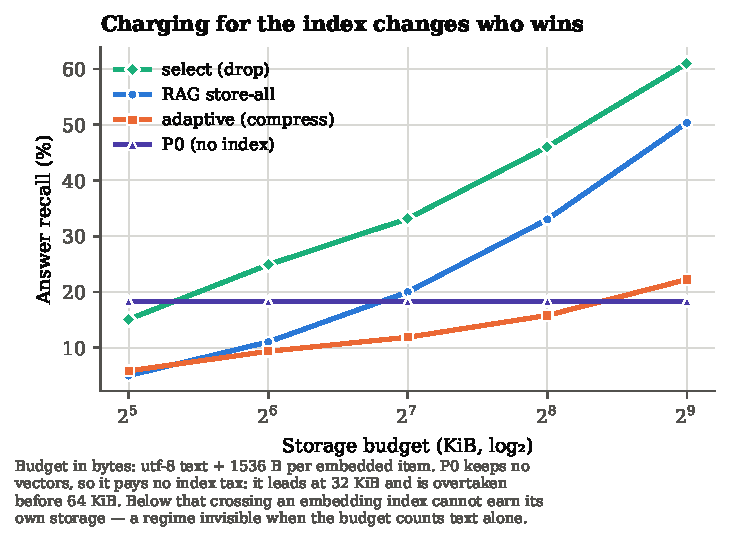
\includegraphics[width=0.85\textwidth]{../paper/figures/fig4_cost_model.pdf}
\caption{Answer recall with the storage budget counted in bytes, the index
included.}
\label{fig:costfig}
\end{figure}

\section{Scorer analysis}
\label{sec:scorer}

If the value lies in the decision, the scorer that makes it is the part worth
improving. Table~\ref{tab:ablation} removes one mechanism at a time. Retrieval
dominates, at $-31.6$ evidence points, and scored eviction is worth 6.4
points. The demotion row shows the same divergence in miniature: removing
demotion costs 11.5 evidence points and gains 7.1 answer points.

\begin{table}[htbp]
\caption[Component ablation at $S=4096$: change from the full system.]{Component ablation at $S=4096$: change from the full system.
$\dagger$: the row on which the two metrics disagree in direction.}
\label{tab:ablation}
\centering
\fontsize{10}{12}\selectfont
% GENERATED by paper/make_tables.py -- do not edit by hand.
\begin{tabular}{@{}lrr@{}}
\toprule
Component removed & $\Delta$ evidence & $\Delta$ answer \\
\midrule
Retrieval (Tier 3) & $-31.6$ & $-28.0$ \\
Demotion on pressure\,$\dagger$ & $-11.5$ & $+7.1$ \\
Scored eviction ($\rightarrow$ FIFO) & $-6.4$ & $-7.4$ \\
Informative compressor & $-4.4$ & $-1.7$ \\
Consolidation merge & $-3.4$ & $-4.8$ \\
Semantic supersession & $-0.3$ & $-0.3$ \\
\bottomrule
\end{tabular}

\end{table}

Table~\ref{tab:scorers} and Fig.~\ref{fig:scorerfig} vary only the scorer.
Three results follow, all significant under clustering. Scoring is worth
doing: the hand-written heuristic gains $+11.19$ answer points over unscored
recency. The LLM judge \cite{zheng2023judge}, however, loses: Qwen2.5-0.5B
reaches 30.9\% against the heuristic's 36.8\%, $-5.87$ points with the
interval excluding zero, at about fifteen minutes of GPU time per corpus
against microseconds for a regular expression. And the headroom is real: a
logistic scorer fitted leave-one-conversation-out reaches 48.3\%, $+11.47$
over the heuristic.

The judge fails because of what it is shown. It rates each turn on its own,
but salience is not a property of a turn on its own: a phone number matters
because someone asks for it later. The fitted scorer sees the same isolated
text but absorbs corpus-level base rates that a per-turn prompt cannot
convey; its strongest single feature is turn length, ahead of every
hand-designed cue.

\begin{table}[htbp]
\caption[Single-component scorer swap at $S=4096$.]{Single-component scorer swap at $S=4096$. Policy, retrieval and
compression fixed; only the scorer varies. P3 is fitted on the other nine
conversations. Run before the scorer fix (Section~\ref{sec:prefix}).}
\label{tab:scorers}
\centering
\fontsize{10}{12}\selectfont
\begin{adjustbox}{max width=\textwidth}\input{../paper/tables/scorers}\end{adjustbox}
\end{table}

\begin{figure}[htbp]
\centering
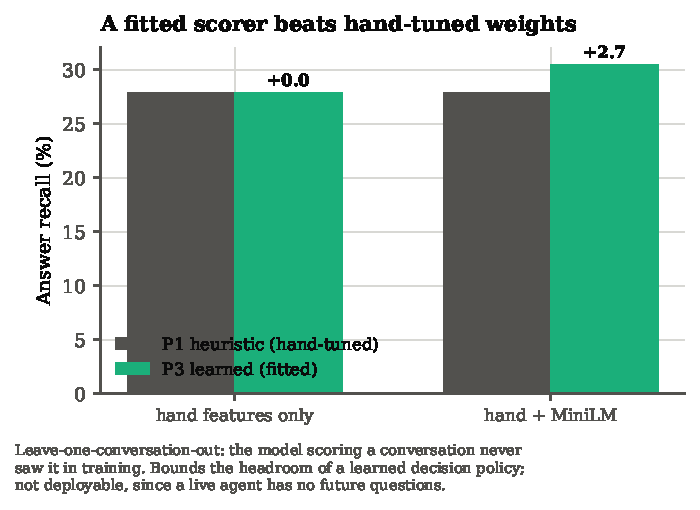
\includegraphics[width=0.8\textwidth]{../paper/figures/fig3_scorer.pdf}
\caption{Answer recall by scorer: recency, heuristic, LLM judge and learned.}
\label{fig:scorerfig}
\end{figure}

\section{A learned scorer across two corpora}
\label{sec:transfer}

LoCoMo's dialogues are generated by an LLM, so a scorer fitted to them may
learn the generator's style rather than what people later ask about. This was
tested on REALTALK \cite{lee2025realtalk}: ten conversations between real
people over 21 days, 8{,}944 turns and 660 questions, of which 160 are
answer-recoverable. Every held-out conversation is scored by three models
that never saw it: trained on the other conversations of the same corpus, on
the other corpus only, or on all 19 other conversations pooled.

Table~\ref{tab:transfer} reports the result. On LoCoMo the pooled scorer
reaches 52.0\% answer recall against the heuristic's 37.5\%, a gain of
$+14.55$ points, and pooling beats same-corpus training by $+3.36$, so adding
a different corpus helped rather than diluted. Transfer works in one
direction only. Trained on REALTALK alone, the scorer still beats the
heuristic on LoCoMo by $+9.09$; trained on LoCoMo alone, it falls below the
heuristic on REALTALK ($-4.38$, n.s.) and is significantly worse than
same-corpus training there.

Because $S=4096$ is the budget of the headline comparison rather than one
chosen for this scorer, Table~\ref{tab:transfer-budget} repeats the pooled run
at four other budgets. On LoCoMo the gain is significant from $S=2048$ to
16384 and largest at 4096. On REALTALK it is significant at $S=8192$
($+16.88$) and 16384. The embedding is what carries across: with the hand
features alone, the pooled scorer is significantly worse than the heuristic on
REALTALK ($-8.75$), because its feature weights encode LoCoMo's style. Logistic
regression was kept after comparing it with boosted trees and a 64-unit MLP:
neither beat it by more than the spread between held-out conversations, and
the trees were much slower.

\begin{table}[htbp]
\caption[Learned scorer on held-out conversations of two corpora, $S=4096$.]{Learned scorer on held-out conversations of two corpora, $S=4096$.
$\Delta$ is answer recall against P1 with 95\% intervals by conversation; bold
excludes zero.}
\label{tab:transfer}
\centering
\fontsize{10}{12}\selectfont
\begin{adjustbox}{max width=\textwidth}% GENERATED by paper/make_tables.py -- do not edit by hand.
\begin{tabular}{@{}lrrrrc@{}}
\toprule
Scorer (trained on) & AUC & Evid. & Ans. & $\Delta$ vs.\ P1 & 95\% CI \\
\midrule
\multicolumn{6}{@{}l}{\emph{LoCoMo} (715 answer-recoverable questions)} \\
\quad RAG (FIFO, no scorer) & -- & 17.8 & 28.1 & --- & --- \\
\quad P1 heuristic & 0.599 & 20.2 & 37.5 & --- & --- \\
\quad P3, same corpus & 0.793 & 32.9 & 48.7 & {\boldmath$+11.19$} & $[+4.72,\, +17.06]$ \\
\quad P3, other corpus only & 0.692 & 30.1 & 46.6 & {\boldmath$+9.09$} & $[+4.53,\, +13.46]$ \\
\quad P3, pooled (shipped) & 0.791 & 34.0 & 52.0 & {\boldmath$+14.55$} & $[+10.40,\, +19.70]$ \\
\multicolumn{6}{@{}l}{\emph{REALTALK} (160 answer-recoverable questions)} \\
\quad RAG (FIFO, no scorer) & -- & 10.5 & 16.9 & --- & --- \\
\quad P1 heuristic & 0.624 & 12.6 & 32.5 & --- & --- \\
\quad P3, same corpus & 0.737 & 18.5 & 38.8 & $+6.25$ & $[-3.01,\, +13.42]$ \\
\quad P3, other corpus only & 0.681 & 11.2 & 28.1 & $-4.38$ & $[-12.50,\, 0.00]$ \\
\quad P3, pooled (shipped) & 0.749 & 17.3 & 36.2 & $+3.75$ & $[-2.92,\, +8.65]$ \\
\bottomrule
\end{tabular}
\end{adjustbox}
\end{table}

\begin{table}[htbp]
\caption[The pooled learned scorer (P3) against the P1 heuristic across the store budget $S$, answer recall (\%).]{The pooled learned scorer (P3) against the P1 heuristic across the
store budget $S$, answer recall (\%). Bold excludes zero.}
\label{tab:transfer-budget}
\centering
\fontsize{10}{12}\selectfont
\begin{adjustbox}{max width=\textwidth}% GENERATED by paper/make_tables.py -- do not edit by hand.
\begin{tabular}{@{}rrrlrrl@{}}
\toprule
& \multicolumn{3}{c}{LoCoMo} & \multicolumn{3}{c}{REALTALK} \\
\cmidrule(lr){2-4}\cmidrule(l){5-7}
$S$ & P1 & P3 & $\Delta$ [95\% CI] & P1 & P3 & $\Delta$ [95\% CI] \\
\midrule
1024 & 15.8 & 19.0 & $+3.22$ $[0.00,\, +6.40]$ & 8.1 & 10.0 & $+1.88$ $[-1.95,\, +5.36]$ \\
2048 & 27.8 & 33.7 & {\boldmath$+5.87$} $[+1.83,\, +9.88]$ & 16.2 & 15.0 & $-1.25$ $[-10.62,\, +3.98]$ \\
4096 & 37.5 & 52.0 & {\boldmath$+14.55$} $[+10.40,\, +19.70]$ & 32.5 & 36.2 & $+3.75$ $[-2.92,\, +8.65]$ \\
8192 & 57.8 & 69.1 & {\boldmath$+11.33$} $[+6.06,\, +16.41]$ & 41.2 & 58.1 & {\boldmath$+16.88$} $[+6.31,\, +26.72]$ \\
16384 & 71.3 & 77.2 & {\boldmath$+5.87$} $[+2.04,\, +10.56]$ & 61.3 & 68.1 & {\boldmath$+6.88$} $[+2.12,\, +12.21]$ \\
\bottomrule
\end{tabular}
\end{adjustbox}
\end{table}

\section{A negative result on LongMemEval}
\label{sec:lme}

The headline was also tested on LongMemEval \cite{wu2024longmemeval}: 94
independent histories of 38--62 sessions each, with the store budget swept so
that LongMemEval was held at LoCoMo's retention (22.1\% against 22.0\%). Here
the heuristic P1-S \emph{loses} to FIFO by 21.0 answer points (95\% CI
$[-33.9,-8.1]$), where LoCoMo gives a gain. The cause is the scorer rather than
the mechanism: the heuristic's separation between evidence and non-evidence
turns reverses sign, from $+0.0476$ on LoCoMo to $-0.0346$ on LongMemEval, so
eviction discards evidence first. The heuristic was written for LoCoMo's
short dialogue lines, and LongMemEval's turns are long prose. An obvious
confound, the share of the context reserved for recent turns, was ruled out:
removing it changed answer recall by exactly zero. This run used the
heuristic before the scorer fix; the learned scorer has not yet been tested on
LongMemEval, and that is listed as future work.

\section{End-task accuracy}
\label{sec:endtask}

Everything so far is context recall, which caps end-task accuracy without
measuring it. To measure it, each assembled context was passed to one fixed
reader, Qwen2.5-1.5B-Instruct-4bit decoding greedily for at most 32 tokens,
and the output was scored with the same normaliser the answer-recall metric
uses, over all 715 answer-recoverable questions, with a closed-book arm (no
memory) and an oracle arm (exactly the cited evidence).

Table~\ref{tab:endtask} and Fig.~\ref{fig:endtask} report the outcome. The
closed-book floor is 1.7\%, so the margin above it is due to the memory layer.
P1-S reaches 18.5\% against RAG's 12.4\%, a realised gap of $+6.0$ points
(95\% CI $[+3.3,+9.1]$), which is 69\% of the $+8.7$-point recall gap between
the same two arms in this run. Accuracy given that the answer was present is
49.4\% for P1-S against 42.3\% for RAG, so P1-S both places the answer in
context more often and assembles contexts the reader uses more successfully.
The oracle converts a complete context into a correct answer 67.3\% of the
time, which locates the remaining headroom in the reader rather than in the
memory layer.

\begin{table}[htbp]
\caption[End-task accuracy through one fixed reader at $S=4096$ over all 715 answer-recoverable questions.]{End-task accuracy through one fixed reader at $S=4096$ over all 715
answer-recoverable questions. Acc.$\mid$present is accuracy on the questions
whose answer reached the context. Run before the scorer fix.}
\label{tab:endtask}
\centering
\fontsize{10}{12}\selectfont
\input{../paper/tables/endtask}
\end{table}

\begin{figure}[htbp]
\centering
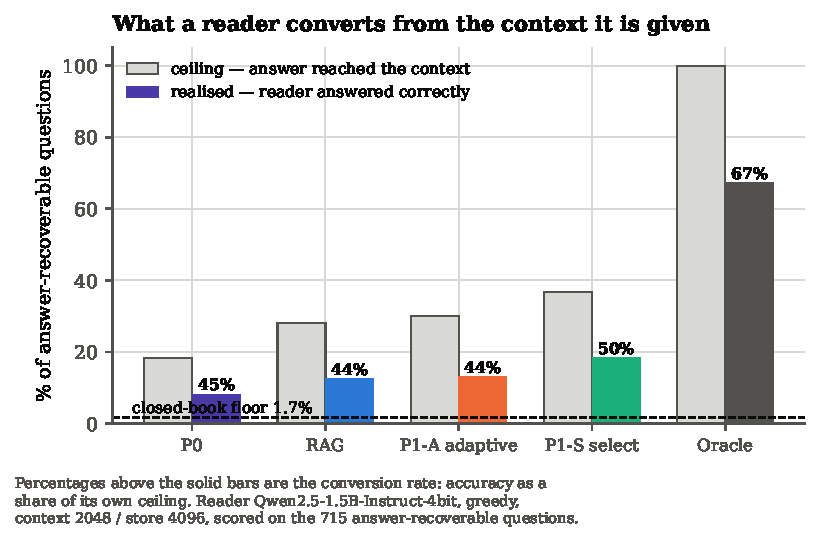
\includegraphics[width=0.8\textwidth]{../paper/figures/fig5_endtask.pdf}
\caption{Reader accuracy by memory policy, with the closed-book floor and the
oracle ceiling.}
\label{fig:endtask}
\end{figure}

Two further runs refine the compression result. Replacing the extractive
compressor with the 1.5B model rewriting each evicted turn gains $+4.06$
answer points over extractive compression (95\% CI $[+0.84,+6.66]$), so part
of the compression loss was the compressor; dropping still wins, 36.8\%
against 34.1\%, at about 1{,}850 times the compute. A scorer learned online
from retrieval feedback, with no labels and no future questions, is
statistically level with the heuristic ($-2.94$, CI $[-7.93,+1.13]$).

\section{Against MemGPT-style and Mem0-style memory}
\label{sec:external}

To compare MemGate with designs in actual use, the memory management of
MemGPT \cite{packer2023memgpt} and Mem0 \cite{chhikara2025mem0} was rebuilt
inside the same harness at the same budgets. The MemGPT-style arm keeps a
recent queue and a searchable archive and folds evicted messages into a
recursive summary that is always in context. The Mem0-style arm writes one
compressed fact per turn with ADD, UPDATE and NOOP and evicts the least
recently touched fact. Neither calls an LLM, so these are the systems' memory
structures rather than their prompts. In the baselines' favour, their
settings were grid-searched on LoCoMo itself at $S=4096$; no MemGate arm was
tuned on these answers.

Table~\ref{tab:external} and Fig.~\ref{fig:external} report the result. The
learned scorer beats both rebuilds at every budget, by $+7.3$ to $+24.6$ points
over Mem0-style and $+11.5$ to $+22.7$ over MemGPT-style, every gap significant.
The untrained P1 heuristic beats MemGPT-style everywhere but loses to the tuned
Mem0-style at $S=4096$, the budget its settings were chosen on. Mem0-style
stops improving at 52.6\% from $S=8192$, because UPDATE replaces a fact with its
nearest neighbour and so discards distinct facts that merely look alike.
MemGPT-style stays within about two points of plain RAG, because its summary
holds gists whose answers were compressed away.

\begin{table}[htbp]
\caption[Answer recall (\%) on LoCoMo against rebuilt MemGPT-style and Mem0-style memory.]{Answer recall (\%) on LoCoMo against rebuilt MemGPT-style and
Mem0-style memory. Bold $\Delta$: the interval by conversation excludes zero.}
\label{tab:external}
\centering
\fontsize{10}{12}\selectfont
\begin{adjustbox}{max width=\textwidth}% GENERATED by paper/make_tables.py -- do not edit by hand.
\begin{tabular}{@{}rrrrrrrr@{}}
\toprule
& & MemGPT & Mem0 & & & \multicolumn{2}{c}{$\Delta$ vs.\ Mem0-style} \\
\cmidrule(l){7-8}
$S$ & RAG & -style & -style & P1-S & P3 & P1-S & P3 \\
\midrule
2048 & 18.3 & 18.7 & 26.4 & 27.8 & \textbf{33.7} & $+1.4$ & {\boldmath$+7.3$} \\
4096 & 28.1 & 30.2 & 44.5 & 37.5 & \textbf{52.0} & {\boldmath$-7.0$} & {\boldmath$+7.6$} \\
8192 & 44.3 & 46.4 & 52.6 & 57.8 & \textbf{69.1} & $+5.2$ & {\boldmath$+16.5$} \\
16384 & 66.4 & 65.7 & 52.6 & 71.3 & \textbf{77.2} & {\boldmath$+18.7$} & {\boldmath$+24.6$} \\
\bottomrule
\end{tabular}
\end{adjustbox}
\end{table}

\begin{figure}[htbp]
\centering
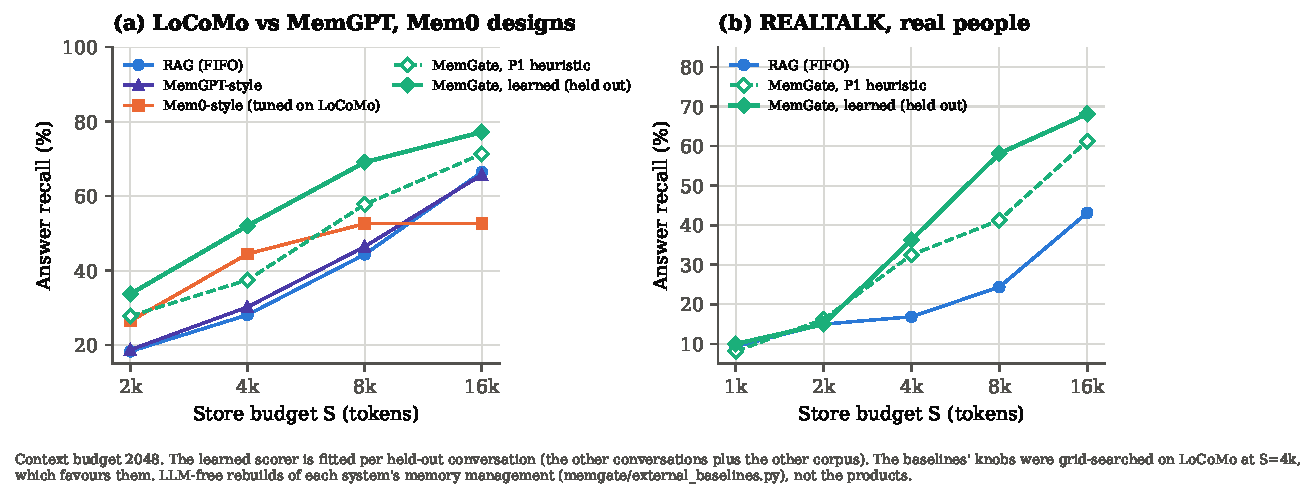
\includegraphics[width=0.8\textwidth]{../paper/figures/fig6_external.pdf}
\caption{Answer recall against the store budget for MemGate and the rebuilt
MemGPT-style and Mem0-style memories.}
\label{fig:external}
\end{figure}

\section{Chats of up to ten million tokens}
\label{sec:scale}

LoCoMo conversations average about 19K tokens. BEAM \cite{tavakoli2026beam}
supplies user--assistant chats of 100K, 500K, 1M and 10M tokens, and MemBench
\cite{tan2025membench} short agent trajectories. Each conversation was scored
by a learned scorer fitted, under five folds by conversation, without it;
BEAM 1M and 10M lie outside its training corpora altogether. The store budget
for BEAM is $S=26{,}000$, about 2.5\% of a 1M-token chat.

Table~\ref{tab:scale} reports answer recall. The learned scorer beats RAG on
all seven corpora with the interval excluding zero, by $+36.5$ points on BEAM
1M and $+46.2$ on BEAM 10M. On a million-token chat RAG keeps only the most
recent turns, so almost nothing it is asked about survives. The one corpus on
which the learned scorer is not the best is MemBench, whose short factual
statements are what the P1 rules were written to find. BEAM answers are mostly
paraphrases, so only a few questions per corpus are answer-recoverable, and
the BEAM 10M row rests on 13 questions.

\begin{table}[htbp]
\caption[Held-out answer recall (\%) at each corpus's store budget, 5-fold by conversation.]{Held-out answer recall (\%) at each corpus's store budget, 5-fold by
conversation. P3$_{12}$: the earlier recipe; P3$_{\mathrm{ship}}$: the shipped
ensemble. Bold: the interval excludes zero. $^\ddagger$PersonaChat validation
dialogues, never trained on.}
\label{tab:scale}
\centering
\fontsize{10}{12}\selectfont
\begin{adjustbox}{max width=\textwidth}% GENERATED by paper/make_tables.py -- do not edit by hand.
\begin{tabular}{@{}lrrrrrlrl@{}}
\toprule
Corpus & $S$ & $n$ & RAG & P1 & P3$_{12}$ & P3$_{12}-$RAG [95\% CI] & P3$_{\mathrm{ship}}$ & P3$_{\mathrm{ship}}-$P3$_{12}$ [95\% CI] \\
\midrule
LoCoMo & 4096 & 715 & 28.1 & 37.5 & 50.3 & {\boldmath$+22.2$} $[+17.5,\, +27.6]$ & 51.9 & $+1.5$ $[-0.2,\, +3.4]$ \\
REALTALK & 4096 & 160 & 16.9 & 32.5 & 36.2 & {\boldmath$+19.4$} $[+7.5,\, +26.4]$ & 36.2 & $0.0$ $[-3.3,\, +3.1]$ \\
BEAM 100K & 26K & 34 & 32.4 & 35.3 & 73.5 & {\boldmath$+41.2$} $[+14.3,\, +67.6]$ & 73.5 & $0.0$ $[0.0,\, 0.0]$ \\
BEAM 500K & 26K & 55 & 32.7 & 32.7 & 63.6 & {\boldmath$+30.9$} $[+16.7,\, +44.8]$ & 61.8 & $-1.8$ $[-10.0,\, +5.8]$ \\
BEAM 1M & 26K & 52 & 13.5 & 11.5 & 50.0 & {\boldmath$+36.5$} $[+21.8,\, +51.0]$ & 50.0 & $0.0$ $[-7.3,\, +8.0]$ \\
BEAM 10M & 26K & 13 & 7.7 & 23.1 & 53.8 & {\boldmath$+46.2$} $[+10.0,\, +76.9]$ & 38.5 & $-15.4$ $[-44.4,\, 0.0]$ \\
MemBench & 2048 & 367 & 76.8 & 97.5 & 95.6 & {\boldmath$+18.8$} $[+14.2,\, +23.7]$ & 97.5 & {\boldmath$+1.9$} $[+0.3,\, +3.8]$ \\
Everyday chat$^\ddagger$ & 1024 & 1762 & 28.8 & 30.4 & 61.4 & --- & 69.0 & {\boldmath$+7.6$} $[+5.9,\, +9.5]$ \\
\bottomrule
\end{tabular}
\end{adjustbox}
\end{table}

\section{Ten times the training data}
\label{sec:retrain}

The scorer that the application first shipped was fitted on 58{,}616 turns.
It was retrained on ten times that, adding BEAM 1M and 10M and MemBench,
594{,}000 turns in all. Each candidate was replayed on held-out conversations
at three to five budgets per corpus, with the folds dealt in three different
orders, 26{,}444 replays in all, under the rule that a shipped model must lose
nowhere.

More data on its own did not help (Table~\ref{tab:retrain}, first column). The
10$\times$ model gained on MemBench but lost evidence recall on BEAM 1M and
500K in every shuffle. A linear model on 399 inputs was short of capacity, not
of data, and the new turns were mostly negatives. Boosted trees, the obvious
source of capacity, lost 8.5 points on LoCoMo and were rejected. Three changes
put it right: weighting corpora within a family by their evidence turns,
adding everyday chat from PersonaChat \cite{zhang2018personachat} as a fifth
family (262{,}876 turns), and averaging the result in logit space with the
earlier model, Eq.~(\ref{eq:ens}). The shipped model is trained on 856{,}876
turns, 14.6 times the original, and has no significant loss on any corpus at
the paper's budgets; it gains $+7.6$ to $+8.2$ answer points on everyday chat.

\begin{table}[htbp]
\caption[Retraining: change against the earlier recipe in three reshuffled fold orders, held out.]{Retraining: change against the earlier recipe in three reshuffled
fold orders, held out. ``App path'' adds the application's chunking, guard
and multi-query retrieval. Bold: the interval excludes zero.}
\label{tab:retrain}
\centering
\fontsize{10}{12}\selectfont
\begin{adjustbox}{max width=\textwidth}% GENERATED by paper/make_tables.py -- do not edit by hand.
\begin{tabular}{@{}llll@{}}
\toprule
& 10x (594K turns) & \multicolumn{2}{c}{Shipped (857K turns)} \\
\cmidrule(lr){2-2}\cmidrule(l){3-4}
Corpus & Evidence & Answer & Evidence \\
\midrule
LoCoMo & $-0.4$, $-0.8$, $-0.2$ & $+1.5$, $-0.3$, $+0.3$ & $+0.1$, $-0.2$, $+0.2$ \\
REALTALK & $+0.1$, $-1.6$, $0.0$ & $0.0$, $0.0$, $+0.6$ & $-0.3$, $-0.8$, $+0.2$ \\
BEAM 100K & $-1.3$, $-0.8$, {\boldmath$-3.7$} & $0.0$, $+2.9$, $-2.9$ & $+1.8$, {\boldmath$+1.8$}, $+0.6$ \\
BEAM 500K & {\boldmath$-5.2$}, {\boldmath$-4.4$}, {\boldmath$-3.0$} & $-1.8$, $+1.8$, $+1.8$ & $+1.6$, $+2.0$, {\boldmath$+2.8$} \\
BEAM 1M & {\boldmath$-5.1$}, {\boldmath$-5.6$}, {\boldmath$-5.3$} & $0.0$, $-1.9$, $+1.9$ & $+0.3$, $0.0$, $-0.4$ \\
BEAM 10M & {\boldmath$-2.3$}, $-2.5$, $-0.5$ & $-15.4$, $0.0$, $-7.7$ & $-1.2$, $-1.8$, $+1.2$ \\
MemBench & {\boldmath$+5.5$}, {\boldmath$+5.8$}, {\boldmath$+6.2$} & {\boldmath$+1.9$}, {\boldmath$+1.9$}, {\boldmath$+2.2$} & {\boldmath$+5.6$}, {\boldmath$+5.9$}, {\boldmath$+6.4$} \\
Everyday chat$^\ddagger$ & --- & {\boldmath$+7.6$}, {\boldmath$+8.2$}, {\boldmath$+8.0$} & {\boldmath$+8.8$}, {\boldmath$+9.1$}, {\boldmath$+9.3$} \\
App path, BEAM 100K & {\boldmath$+6.1$}, $+4.2$, $+6.0$ & {\boldmath$+11.8$}, {\boldmath$+11.8$}, $+8.8$ & {\boldmath$+12.4$}, {\boldmath$+11.5$}, {\boldmath$+11.9$} \\
App path, LoCoMo & $-0.5$, $-0.7$, $-0.2$ & $+1.5$, $0.0$, $+0.4$ & $+0.3$, $+0.1$, $+0.5$ \\
App path, REALTALK & $+0.7$, $+0.3$, $-0.3$ & $+3.1$, $+1.9$, $+0.6$ & $+0.5$, $-0.1$, $0.0$ \\
\bottomrule
\end{tabular}
\end{adjustbox}
\end{table}

\section{Stress and scale through the application}
\label{sec:stress}

The complete pipeline was also tested the way a user meets it. Whole BEAM
chats were typed into the application one message at a time, exactly as its
page sends them, at $S=26{,}000$, and each answerable question was then asked
as a message. Table~\ref{tab:appbeam} reports the result: on million-token
chats, which MemGate holds at about 2.5\%, the answer reaches the reader for
51.9\% of questions against 19.2\% for RAG and 9.6\% for a sliding window. The
store never exceeded $S$, and a message took 0.49\,s on average on a shared
4-core machine.

\begin{table}[htbp]
\caption{Whole BEAM chats typed into the application one message at a time,
$S=26{,}000$; answer recall (\%).}
\label{tab:appbeam}
\centering
\fontsize{10}{12}\selectfont
\begin{adjustbox}{max width=\textwidth}% GENERATED by paper/make_tables.py -- do not edit by hand.
\begin{tabular}{@{}lrrrrrrlr@{}}
\toprule
Chats & $N$ & M tok. & $n$ & P0 & RAG & MemGate & $\Delta$ vs.\ RAG [95\% CI] & McNemar $p$ \\
\midrule
BEAM 1M & 33 & 1.07 & 52 & 9.6 & 19.2 & \textbf{51.9} & {\boldmath$+32.7$} $[+19.2,\, +46.3]$ & $9.1\!\times\!10^{-4}$ \\
BEAM 500K & 33 & 0.52 & 55 & 12.7 & 30.9 & \textbf{65.5} & {\boldmath$+34.5$} $[+19.6,\, +49.1]$ & $3.1\!\times\!10^{-4}$ \\
\bottomrule
\end{tabular}
\end{adjustbox}
\end{table}

Much of the gap comes down to where the evidence sits (Table~\ref{tab:age}).
RAG forgets oldest first, so for evidence in the first third of a
conversation it keeps the answer 8--9\% of the time; the untrained heuristic
keeps 20--33\%, and the learned scorer more. For evidence in the last third
RAG is competitive, since recency is then the right rule.

\begin{table}[htbp]
\caption[Answer recall (\%) by the position of a question's evidence, $S=4096$.]{Answer recall (\%) by the position of a question's evidence,
$S=4096$. $^\ast$In-sample on both corpora.}
\label{tab:age}
\centering
\fontsize{10}{12}\selectfont
% GENERATED by paper/make_tables.py -- do not edit by hand.
\begin{tabular}{@{}llrrrr@{}}
\toprule
Corpus & Evidence in & $n$ & RAG & P1 & P3$^\ast$ \\
\midrule
LoCoMo & first & 262 & 9.2 & 33.2 & 51.9 \\
 & middle & 225 & 14.2 & 38.2 & 53.8 \\
 & last & 228 & 63.6 & 41.7 & 54.4 \\
\midrule
REALTALK & first & 86 & 8.1 & 19.8 & 33.7 \\
 & middle & 45 & 11.1 & 40.0 & 55.6 \\
 & last & 29 & 51.7 & 58.6 & 65.5 \\
\bottomrule
\end{tabular}

\end{table}

People rarely ask one clean question per message. When each LoCoMo question
was buried in 150--450 words of other chat, using the whole message as the
query dropped answer recall from 53.1\% to 30.3\%; making each question its
own query with interleaved rankings recovers 49.8\%.

The same tests found six input-handling bugs, each now pinned by a test:
half of an emoji in one message made every later save of that chat fail; a
300\,KB Word file that unzips to 300\,MB used 3.8\,GB of memory; deeply nested
JSON dropped the connection; request bodies had no size limit; a message of
only invisible characters was accepted; and a locked PDF gave an unclear
error. A load test found one more: under bursts, the server's accept queue of
five reset 314 of 2{,}000 requests from 200 simultaneous visitors. With a queue
of 256 the same test completes with no errors in 25\,s, and a single chat of
5{,}000 messages stays at 4{,}093 of its 4{,}096 tokens, at 0.12\,s per message.

\section{Standards followed}
\label{sec:standards}

The following standards and practices were adhered to in building and
testing the system and in validating its results.
\begin{itemize}
\item \textbf{IEEE Std 754 (floating-point arithmetic).} All embeddings and
  model weights are IEEE~754 single-precision (\texttt{float32}) values;
  the 1{,}536-byte cost of a vector in Eq.~(\ref{eq:cost}) is $384\times4$
  bytes of this format.
\item \textbf{ISO/IEC/IEEE 29119 (software testing) and IEEE Std 1012
  (verification and validation).} Testing follows their structure: unit
  tests for each module, integration tests through the application's API,
  and a benchmark-level validation test that replays LoCoMo and compares it
  with the published numbers; regression tests pin every fixed defect.
\item \textbf{ISO/IEC/IEEE 29148 (requirements engineering).} The scope,
  in-scope and out-of-scope items and the measurable objectives of
  Chapter~\ref{ch:intro} were written as verifiable requirements, each
  checked by an experiment or a test.
\item \textbf{Unicode and UTF-8 (RFC 3629).} All text is stored as UTF-8 and
  NFC-normalised; control characters, zero-width marks and bidirectional
  overrides are removed on input.
\item \textbf{RFC 9110 (HTTP semantics) and RFC 8259 (JSON).} The
  application's server uses standard HTTP methods and status codes and
  exchanges JSON.
\item \textbf{Statistical practice.} Paired bootstrap confidence intervals
  clustered by conversation \cite{efron1993bootstrap,cameron2008cluster} and
  exact McNemar tests \cite{mcnemar1947,dietterich1998tests}; a result is
  claimed only when its interval excludes zero.
\item \textbf{Reproducibility.} Every model is a pinned local copy; every
  table is generated from committed result files; and the leakage invariant
  (no decision may read an evaluation label) is enforced by tests
  \cite{kaufman2012leakage,kapoor2023leakage}.
\end{itemize}

\section*{Summary}
Once the store is bounded, deciding what to forget is worth $+9.37$ answer
points over FIFO, while compressing instead of dropping costs $7.13$; no
rate--distortion crossover appears up to $182\times$; and counting the index
in bytes reverses the ranking below about 40\,KiB. An LLM judge loses to a
heuristic, but a learned scorer beats the heuristic by $+14.55$ points on
held-out conversations, transfers from human to generated dialogue, beats
MemGPT-style and Mem0-style memory at every budget, and keeps the answer for
51.9\% of questions on million-token chats against 19.2\% for retrieval. Two
results are negative: the heuristic fails on LongMemEval, and ten times the
data alone did not improve the scorer.
